\chapter{Evaluation of Visualization Methods}
\label{Chapter4}

In this chapter, we use the prototype implemented in chapter \ref{Chapter3} to conduct an experiment to evaluate the five visualization methods proposed in section \ref{VisualizationMethods}.

%------------------------------------------------------------------------------

\section{Evaluation Condition}

The experiment only focuses on the understandability evaluation. Other things like realtimeness, accuracy, and robustness as described in section \ref{VisualizationRequirements} are not considered.

Students of about 20--30 years old are invited to use the system with the five visualization methods. After that, each user is asked to rank the understandability of each visualization method in five levels of ranking points (1: worst, 5: best). Each user is forced to give unique ranking points across all five methods.

We have conducted the experiment outside the building of the College of Engineering Systems, at the area as in figure \ref{fig:VolumeMethod} and \ref{fig:SceneModel}:

\begin{itemize}
	\item Use the ``two keyframes'' method in section \ref{MapInitializing} to initialize the PTAM map.
	\item Each user points the mobile camera at the wall and see the visualized viewing field of a virtual camera. The user can change the position and/or orientation of the mobile. They can also walk around the area.
	\item The iPhone is used. The video frame size is 304 x 400, and is enlarged to 320 x 421 to fit the width of the screen. It operates at about 7 frame-per-second.
\end{itemize}

Figure \ref{fig:ExperimentScreenshot} shows a screenshot of the arrow visualization method. The users can use button 1--5 to switch among visualization methods, and button M to toggle between real and map viewing mode. The A button is for administration task, not used by the users.

\begin{figure}[htbp]
	\centering
	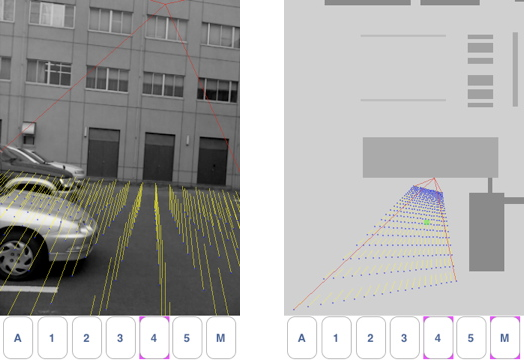
\includegraphics[width=14cm]{./Primitives/experiment_screenshot.png}
	\rule{35em}{0.5pt}
	\caption[Evaluation experiment screenshot]{Evaluation experiment screenshot of the arrow visualization method in real viewing mode (left) and map viewing mode (right)}
	\label{fig:ExperimentScreenshot}
\end{figure}

%------------------------------------------------------------------------------

\section{Result and Discussion}

The result is shown in table \ref{tb:ExperimentResult}. The numbers inside parentheses are points given by the users. The outside numbers are the average of the inside numbers.

\begin{table}[tb]
	\begin{center}
		\caption{Result of the evaluation experiment of visualization methods}
		\label{tb:ExperimentResult}
		\begin{tabular}{|c|c|c|c|c|}
			\hline
			Method    & Understandability \\
			\hline
			Volume    & 1.0 (1 1 1) \\
			Shadow    & 3.0 (3 4 2) \\
			Contour   & 2.7 (2 2 4) \\
			Arrow     & 3.3 (4 3 3) \\
			Animation & 5.0 (5 5 5) \\
			\hline
		\end{tabular}
	\end{center}
\end{table}

The winner of understandability is the animation method. A good visualization method is the one in which CG objects used to visualize the viewing fields do not occlude the scene. Moving objects do not occlude the scene over time, hence the animation method gives the best understandability. Moreover, this method also points out where the surveillance camera. On the contrary, viewing field visualized by the volume method is the worst because the CG object usually occlude large parts of the screen.

The ranking points of other categories are about the same. This is because they are based on the same prototype system, hence they should share the same characteristics specified by each category. Moreover, the users have evaluated the system as very good. We have only conducted the experiment in a small outdoor area. More extensive experiments in various conditions, such as larger areas, different lighting conditions etc. should be conducted before more solid conclusion could be made. In those conditions, methods with non-animated CG objects may be of less understandability because the CG objects may have similar color with the color of the texture of the real scene.

A good gene is usually a mixture of pure gene or other mixed gene. Likewise a good visualization can be a combination of various methods. In the future we should try to combine the methods to find ones better than the current animation method.

Although the experiment is still simple with few evaluators, they all agree that of the five methods, animation method gives the best understandable visualization. This method is preferable because it does not occlude the scene and gives the users the visualization of both positions and viewing fields of the surveillance cameras.

The result is largely affected by the way we draw the visual aids. In previous experiments, we did not draw the four straight lines as described at the begin of section \ref{VisualizationMethods}, and 

The result may also affected by the color of the visual aids.
Color of
Mau sac anh huong qua
=> future: cho phep user customize interactively

0.5*source color + 0.5*destination color
	
